\subsection{Сверточные нейронные сети (CNN)}
Созданные для задач компьютерного зрения сверточные нейронные сети
\cite{LeCun:1, LeCun:2, LeCun:3} были
достаточно продуктивно применены и в других сферах глубокого обучения,
в том числе и NLP (natural language processing, 
обработка естественного языка).
Использование их достигло максимума в ответ на
ограниченность применения полносвязных сетей для обработки данных с сеточной топологией \cite{Goodfellow}.
\subsubsection{Операция свертки}
\textit{Определение:} Пусть $u, v: \ \mathbb{R}^{n} \to \mathbb{R}$ -- две функции, интегрируемые относительно меры Лебега
    на пространстве $\mathbb{R}^{n}$. Тогда функция  $u * v: \ \mathbb{R}^n \to \mathbb{R}$ называется сверткой
    и определяется соотношением:
    \[(u * v) (x) := \int\limits_{\mathbb{R}^{n}} u(y)v(x-y)dy,\]
    где $y$ иногда называют давностью, $u$ -- входом, $v$ -- ядром свертки (kernel). Результат
свертки именуется картой признаков (feature map).
В задаче классификации текстов в силу плоского векторного представления слов будем рассматривать
одномерную свертку. Для $n = 1$ формула примет вид:
\[(u * v) (x) := \int\limits_{-\infty}^{\infty} u(y) v(x-y)dy\]
Кроме того, задача представляет собой конечный, дискретный случай, значит, окончательный вид формулы:
\[(u * v) (x) := \sum\limits_{y = 0}^{K} u (y) v(x-y),\]
%! проверить K
где K -- размер ядра.

Для иллюстрации операции свертки рассмотрим функции $u, v$ как сигналы рис. \ref{fig:cnn1}.
\begin{figure}[ht]
    \centering
    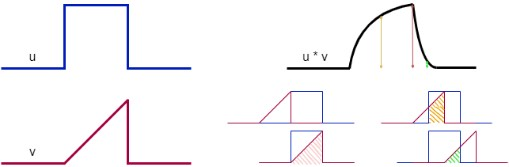
\includegraphics[scale=2]{convolution.jpg}
    \caption{Операция свертки между двумя сигналами $u,v$}
    \label{fig:cnn1}
%! добавить названия рисунков
\end{figure}
Сдвигая ядро $v$ относительно входного сигнала $u$ и, посчитав скалярное произведение векторов, 
получим сходство фрагмента сигнала с ядром, что и является результатом свертки.
\subsubsection{CNN для работы с изображениями}
Для изображений характерно матричное представление, 
каждому элементу которого соответствует значение пикселя. 
На рис. \ref{fig:cnn2}
приведен случай с изображением размерности $5 \times 5 \times 1$.  
\begin{figure}[ht]
    \centering
    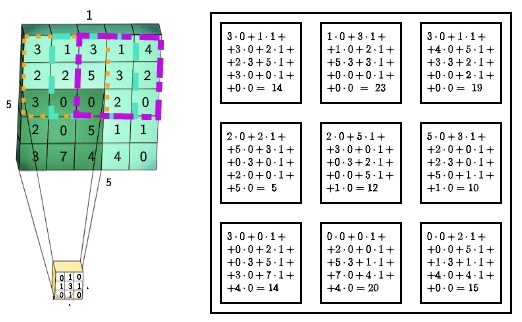
\includegraphics[scale=1]{convolution_images.png}
    \caption{Пример операции свертки для изображения $5\times 5\times 1$ с ядром свертки $3\times 3\times 1$}
    \label{fig:cnn2}
\end{figure}
Ядро свертки (размерности $3 \times 3 \times 1$) прикладывается к каждому фрагменту изображения с задаваемым шагом (stride). 
На Рис. \ref{fig:cnn2} приведен пример со значением шага, равным единице.
Видно, что каждый нейрон связан лишь с частью пикселей, если речь идет о первом сверточном слое или нейронов, 
для последующих слоев (это свойство называют разреженной связностью). Необходимым становится обучение лишь значений ядер свертки, 
что значительно меньше, чем в случае традиционных нейронных сетей (полносвязных).
\subsubsection{Одномерные CNN для работы с текстами}
Как уже было сказано ранее, слова (после векторизации) представляют собой плоские вектора. Поэтому для задач обработки естественного 
языка применяются одномерные сверточные нейронные сети. Токены (в рассматриваемом случае, слова), представленные в векторной форме,
конкатенируются в матрицу текста.
Затем выбирается $k$ строк матрицы, которые вытягиваются в плоский вектор. К нему прикладывается (берется скалярное произведение) 
одномерное ядро размерности $k \cdot s$, где $s$ -- размерность вектора токена. Этот процесс иллюстрирован на рис. \ref{fig:cnn31} 
и рис. \ref{fig:cnn32}. 
\begin{figure}[H]
    \centering
    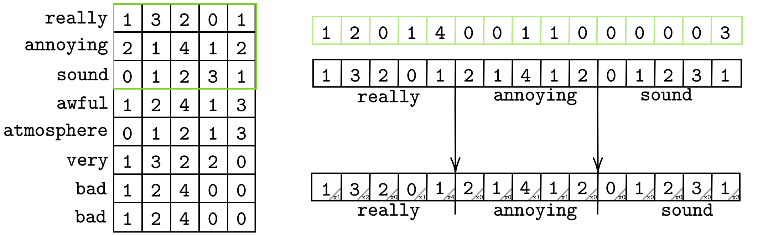
\includegraphics[scale=1.5]{convolution_text_1.png}
    \caption{Применение свертки для извлечения признаков из текста}
    \label{fig:cnn31}
\end{figure}
Двигаясь таким образом по матрице текста, можно получить столбец значений – результатов операции одномерной свертки. 
Для получения большего количества столбцов, которые, в свою очередь, образуют матрицу признаков, используется несколько ядер.
\begin{figure}[H]
    \centering
    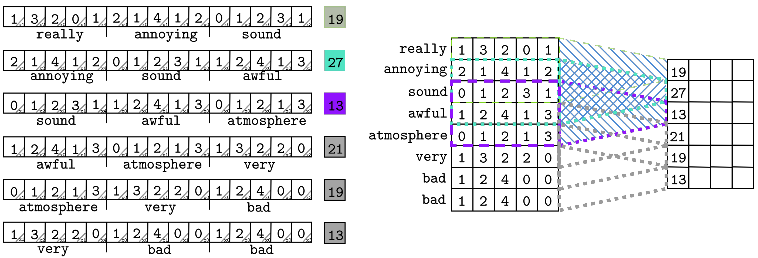
\includegraphics[scale=1.5]{convolution_text_2.png}
    \caption{Применение свертки для извлечения признаков из текста}
    \label{fig:cnn32}
\end{figure}
После применения операции свертки как для изображений, так и для других структур, в том числе и текстов,
 возможно применение слоя субдискритизации (Pooling, подвыборки). Пулинг работает подобно сверточному слою, 
 однако вместо скалярного произведения применяет другие функции на фрагменты, 
 например, возвращает максимальный или средний выходы в прямоугольной окрестности
  (max-пулинг \cite{Zhou:1} и average-пулинг соответственно). \\Max-Pooling:
  \[f_{MP} = \max\limits_{i} x_{i}.\] 
  Average-Pooling:
  \[f_{AP} = \frac{1}{n} \sum\limits_{i=1}^{n}x_{i}.\]
  \bigskip\par
  Логика употребления слоя пулинга заключается в том, что выявленные сверточным слоем закономерности избыточны 
  в своей подробности, значит, возможно уплотнение до менее подробного результата. Однако, если в задаче необходимо 
  сохранять точную пространственную информацию, применение пулинга по всем признакам существенно увеличивает ошибку модели,
  что исследовано экспериментально \cite{Szegedy2014}. Сверточный слой и слой пулинга, следующий за ним, образуют сверточный блок.
   Чем больше количество сверточных блоков, тем более абстрактной или высокоуровневой становится карта признаков.
   \bigskip\par
Заключим, что сверточная нейронная сеть достаточно успешно решает задачу извлечения признаков из данных.
 Экстраполируем этот вывод на одномерную плоскость для работы с текстами: сверточные нейронные сети, извлекая закономерности в текстовых данных, 
 способны различать контекст. Причем ширину контекста можно приблизительно идеализировать шириной рецептивного поля (или пятна восприятия). 
 На рис. \ref{fig:cnn4} ширина рецептивного поля на первом слое равна трем, а ширина рецептивного поля на втором слое равна четырем, 
 таким образом происходит расширение контекста. Однако всё же речь идет о, с точки зрения языка, маленьких паттернах, словосочетаниях 
 и коротких фразах. Для масштабного и более полного моделирования языка необходимо делать очень глубокие сети, что неминуемо приводит к
 увеличению числа обучаемых параметров.
\begin{figure}[H]
    \centering
    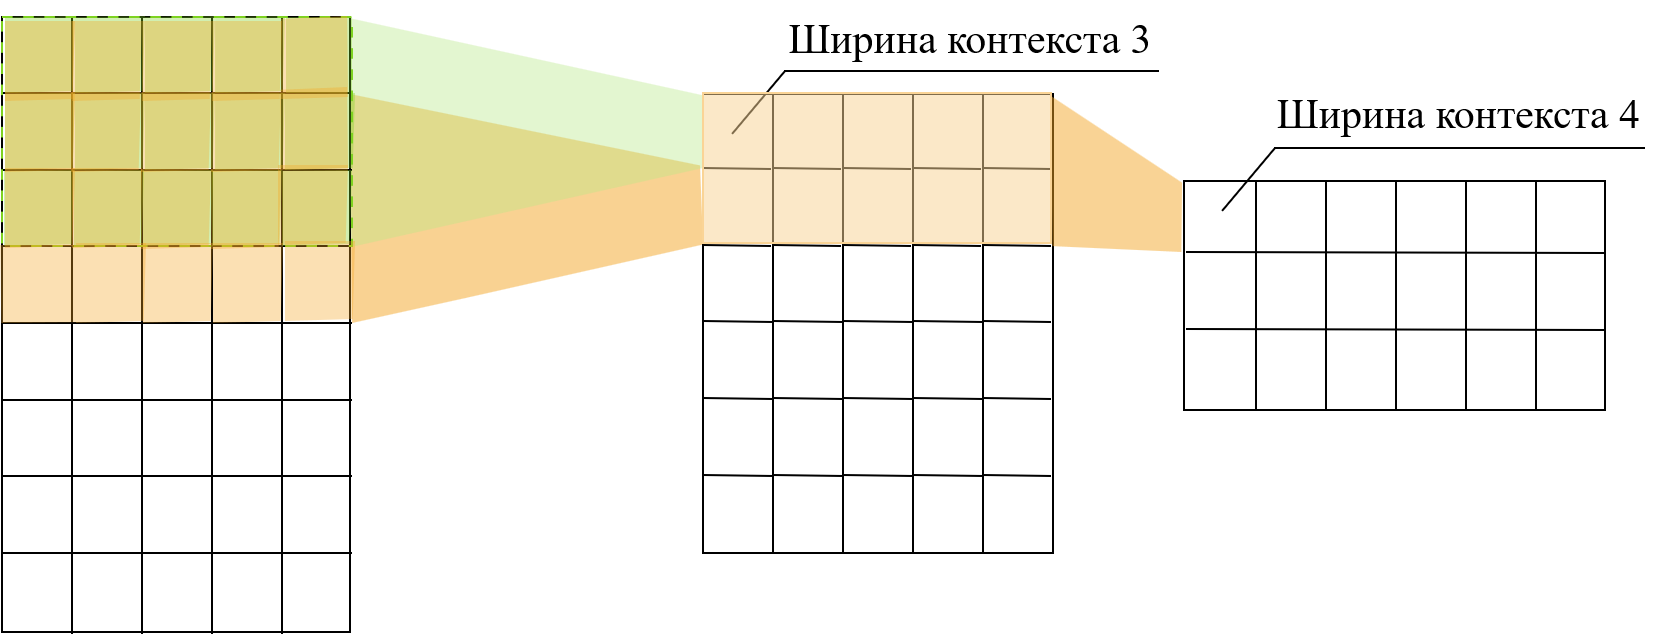
\includegraphics[scale=0.5]{context_width}
    \caption{Ширина рецептивных полей}
    \label{fig:cnn4}
\end{figure}
Существует другой способ увеличения ширины контекста, который, так же как и пулинг, является спорным в употреблении в некоторых условиях задач:
прореживание (dilation) \cite{Srivastava:1}. Заключается он в применении свертки к фрагменту, из которого удалена часть элементов. Например,
возьмем $k$ строк не подряд, а через одну, но значит это то, что мы пропускаем каждое второе слово, что не может однозначно сказаться на решаемой проблеме.
\bigskip\par
Для решения задачи классификации после череды сверточных блоков (сверточный слой + слой пулинг) конечную карту признаков любой размерности, в зависимости от предыдущих слоев,
необходимо растянуть в вектор и подать в полносвязный слой с функцией активации SoftMax (для классификации $n$-классов, $n\in\mathbb{N}$) или Sigmoid (для бинарной классификации),
чтобы получить вероятности классов. 
\bigskip\par
Формула размерности карты признаков, учитывая всевозможные преобразования, после применения сверточного слоя или пулинга:
\[L_{\text{вых}} = \frac{L_{\text{вх}} + 2 \cdot \mathrm{padding} - \mathrm{dilation} \cdot (\mathrm{kernel\textunderscore size} -1) -1}{\mathrm{stride}} + 1,\]
где $\mathrm{padding}$(замощение) -- параметр, используемый в случае, когда есть необходимость в сохранении размерности при выполнении свертки или пулинга: недостающие элементы
для этого заполняются нулями. 
\subsubsection{Преимущества, недостатки и способы борьбы с ними}
% ? редактировать!!!
Сверточные нейронные сети хорошо находят закономерности в пространственных данных. Для текста эти зависимости именуются контекстом, идеализацией которого является ширина рецептивных полей сети. 
Так как вычислительные ресурсы ограничены, то построение очень глубоких сетей такой архитектуры затруднительно.
Ширина рецептивных полей сверточных нейронных сетей позволяет определять частичный контект текстовой информации:
прореживание и пулинг дают возможность увеличить контекст, однако их использование требует достаточной осторожности и может привести к росту ошибки. 
Это не мешает отлично справляться с задачей классификации текстов одномерным сверточным сетям, что доказывают результаты. Но всё становится значительно хуже при попытках моделирования языка. К тому же,
сверточные нейронные сети, как и традиционные, требуют входные данные фиксированной длины, что накладывает ограничение на плоское пространство текстов. В среднем, такие ограничения не оказывают критичного влияния, 
но объемные текста могут нести важные для классификации детали в той своей части, которую не покрывает выбранный масштаб анализа. 